In this section, we describe a non-recursive implementation of the work function algorithm utilizing a min cost flow problem formulation, as described in~\cite{mcfp2011}. A formal reduction proof of this formulation is provided in~\cite{mcfp2011}. We do not provide this proof here, rather we provide an overviewing explanation of the general idea that the algorithm attempts to follow. A similar approach can be used for an implementation of an optimal offline algorithm, and is described in the cited artice.

\subsubsection*{Min-Cut Max-Flow Formulation}
For a given work function $w_{\sigma_i}(C_i)$ we have four groupings of nodes, each representing different structures from the underlying work function algorithm, along with a source node $s$ and a sink node $t$. The first set of nodes are labeled $S = \{s_1 ... s_k\}$ representing the initial server configuration, $C_0$. We additionally have a set of nodes $S' = \{s'_1 ... s'_k\}$ representing the final configuraiton, $C_i$. The last two sets, $R = \{r_1 ... r_i\}$ and $R' = \{r'_1 ... r'_i\}$ together represent the request sequence. Each node in $S$ is connected to the source node $s$ with a weight of $0$.

We make a distinction between the subscripts $j$ and $l$ indicating arbitrary servers or requests, and the subscripts $k$ (indicating the $k$th server) and $i$ (indicating the latest request seen). Now, each node in $S$ is connected to each node in $S'$ with a weight of $d(s_j, s'_l)$ the distance between the two points in the metric space. Each node in $S$ is also connected to each node in $R$ with a weight of $d(s_j, r_l)$. Each node $r_j \in R$ is connected \textit{only} to it's corresponding node $r'_j\in R'$, with a weight of negative infinity (in practice, this is a suffuciently large negative weight $-L$). Each node $r'_j \in R' - r'_i$ is connected to each $r_l \in R$ where $l > j$, with a weight of $d(r_j, r_l)$. Additionally, each node $r' \in R'-r'_i$ is connected to each node $s'_l \in S'$ with a weight of $d(r'_j, s'_l)$. The node $r'_i$ is connected to $t$ with a weight of $0$. Finally, we compute a value $X$ such that:

\begin{equation*}
    X = \frac{1}{k-1} \Sigma_{j=1}^{k} d(s'_j, r_i)
\end{equation*}

And connect each $s' \in S'$ to $t$ with a weight of $X-d(s', r_i$). Each arc in this graph has a maximum flow of $1$, clearly making the min-cut equal to $k$ (if we cut between $s$ and nodes in $S$). This flow can be seen in an example network in fig.~\ref{fig:mcfp}.

%create a figure
\begin{figure}[h]
    \centering
    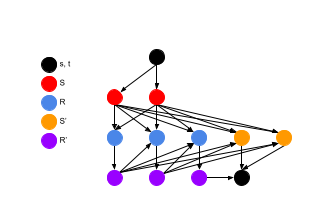
\includegraphics[width=0.5\textwidth]{images/mcfp.png}
    \caption{Min-Cut Max-Flow for Work Function with k=2 and i=3}
    \label{fig:mcfp}
\end{figure}

\subsubsection*{Explanation of the formulation}
When the maximum flow is achieved, we are guarunteed to have flow passing through every node in $S$ due to the min-cut between node $s$ and nodes in $S$. The min cost ensures that we have flow passing through every node in $R$ and $R'$, because of the large negative weight between the two sets. Finally, since $r'_i$ is only connected to $t$, there will be some node $s' \in S'$ that has no flow going to $t$. This will indicate the optimal server to move to service the request $r_i$. Since each flow in the network is $1$, we can break down the network and follow each flow individually. A flow passing through some server $s_j \in S$ indicates the server $j$ that starts at this initial location. If this server passes through some request $r_l$ to $r'_l$, this indicates the server $j$ servicing the $l$th request. Finally, the server will either go to some node $s'$ in the current configuration, or will go to $r'_i$. Going to $s'_l$ indicates it goes to that final location, and going through $r'_i$ indicates that it is the server which services the next request. It is worth noting that this provides a solution to \textit{one} step of the work function algorithm. Whenever we get a new request, we must reconstruct this graph with the additional request added, and recompute a new solution.

\subsubsection*{Finding the cost}

We follow the process described in~\cite{mcfp2011} for solving the minimum cost flow problem. We begin with a null flow through the graph, and then proceed with $k$ iterations each adding a flow of 1 traversing through the graph. 

Each iteration, we find the minimum cost flow through the graph using a modified Bellman-Ford algorithm to ensure that we both get the minimum cost possible, and the capacity of the flow is not exceeded for any arc. We then reverse both the flow and the cost along the arcs traversed by this flow for all following iterations. This process is repeated until we have $k$ flows through the graph. This means that when the first flow is passed through, all nodes in $R$ and $R'$ will be passed through and have their flows and costs reversed, as this minimizes the cost (due to the large negative weight between $R$ and $R'$). Following this, flows may go directly from nodes in $S$ to nodes in $S'$, or they may go through nodes in $R$ and $R'$, but will not re-pass through the $r_j$ to $r'_j$ connections, as these will have very large costs associated with them. Traversing from the set $R'$ to the set $R$ will only involve nodes $r'_j$ and $r_l$ where $j \neq l$. This is because the large negative weight has been reversed, and is now a large positive weight.